\section{Inference memory and attention variants}

\begin{frame}{KV Cache Memory}
  \begin{columns}[T,onlytextwidth]
    \column{0.52\textwidth}
    \begin{itemize}\itemsep0.32em
      \item[\textcolor{red}{$\blacktriangleright$}] While generating (one token per forward pass), each new token needs the key and value tensors of all earlier positions; caching them avoids recomputation, one cache per layer.
      \item[\textcolor{red}{$\blacktriangleright$}] Serving memory consists of model weights plus the KV cache, and under batching every request needs its own cache, often the limiting factor before weights.
      \item[\textcolor{red}{$\blacktriangleright$}] Cost grows linearly with batch size and context length, capping throughput and long-context use; MQA and GQA target this directly.
    \end{itemize}

    \column{0.45\textwidth}
    \centering
    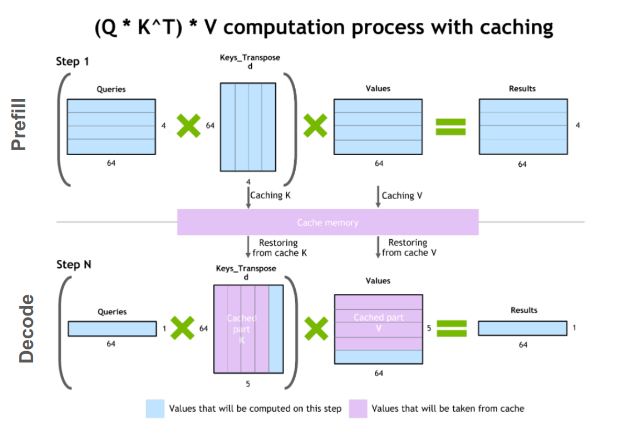
\includegraphics[width=0.8\linewidth,height=0.72\textheight,keepaspectratio]{images/inference-optimisation/nvidia_blog_kv_caching_figure1.png}\\[-0.2em]
    {\scriptsize Illustration of the key-value caching mechanism. Verma \& Vaidya, NVIDIA Technical Blog (2023).}
  \end{columns}
\end{frame}

\begin{frame}{MHA, MQA, GQA: shrinking the KV cache}
  \centering
  
\includegraphics[width=0.95\textwidth,height=0.72\textheight,keepaspectratio]{images/transformers-2017-v-2026/gqa_paper_page_2.png}
  {\scriptsize
    \begin{itemize}
      \item \textbf{Multi-head attention (MHA)}: $H$ separate query, key, and value heads.
      \item \textbf{Multi-query attention (MQA)}: single shared key and value heads for all query heads.
      \item \textbf{Grouped-query attention (GQA)}: shares key and value heads for each \textit{group} of query heads.
      \item GQA conceptually interpolates between multi-head and multi-query attention.
    \end{itemize}
  }
  {\scriptsize \textit{Reference:} Ainslie et al., ``GQA,'' \href{https://arxiv.org/abs/2305.13245}{arXiv:2305.13245}, Figure~2.}
\end{frame}

\begin{frame}{Multi-Head Latent Attention (MLA)}
  \begin{itemize}\itemsep0.15em
    \item MQA and GQA shrink the cache by sharing key and value heads; aggressive sharing costs quality.
    \item MLA (DeepSeek-V2, 2024) instead compresses keys and values into one low-rank latent per token, caches the latent rather than per-head keys and values, and reconstructs them at attention time.
    \item Expressivity stays close to full MHA with a far smaller cache: DeepSeek-V2 reports 93.3\% less KV memory than DeepSeek 67B, already a GQA model. Used across the DeepSeek family (V2, V3, R1).
  \end{itemize}
  \centering
  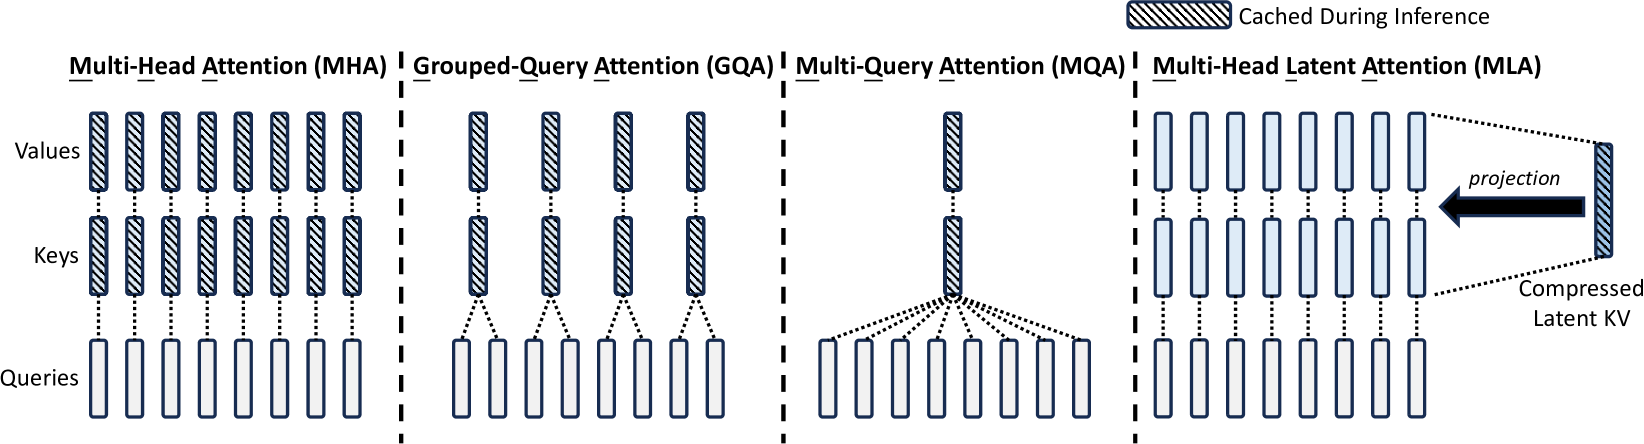
\includegraphics[width=0.85\textwidth,height=0.28\textheight,keepaspectratio]{images/transformers-2017-v-2026/deepseek_v2_mla_vs_mha_gqa_mqa.png}\\[0.15em]
  {\scriptsize DeepSeek-AI, ``DeepSeek-V2: A Strong, Economical, and Efficient Mixture-of-Experts Language Model,'' \href{https://arxiv.org/abs/2405.04434}{arXiv:2405.04434}, Figure 3.}
\end{frame}

\begin{frame}{Sliding-Window and Hybrid Attention}
  \begin{itemize}\itemsep0.15em
    \item Sliding-window attention (Mistral 7B, 2023): each token attends only to the previous $W$ positions ($W = 4096$ in Mistral), capping the per-layer KV cache at $W$ entries no matter how long the context grows.
    \item Information still travels further than $W$: after $L$ layers the receptive field reaches $L \times W$ tokens (32 layers $\times$ 4096 $\approx$ 131k in Mistral 7B).
    \item The 2026 pattern is hybrid: stacks alternate windowed layers with occasional full-attention layers, keeping long-range retrieval while most layers stay cheap. Gemma~2 alternates 1:1, Gemma~3 uses five local layers per global one, and GPT-OSS alternates banded and dense blocks.
  \end{itemize}
  \centering
  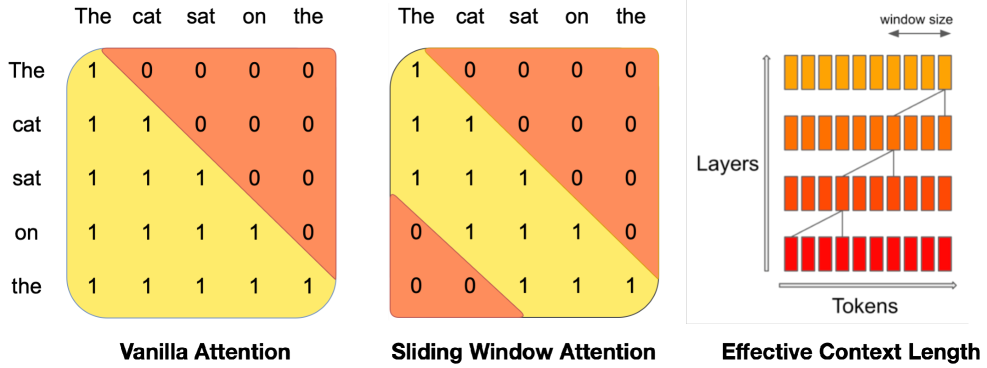
\includegraphics[width=0.72\textwidth,height=0.27\textheight,keepaspectratio]{images/transformers-2017-v-2026/mistral_sliding_window_attention.png}\\[0.15em]
  {\scriptsize Jiang et al., ``Mistral 7B,'' \href{https://arxiv.org/abs/2310.06825}{arXiv:2310.06825}, Figure 1.}
\end{frame}

\begin{frame}{Decoder-only LLMs (post-2017 trend)}
  \begin{itemize}\itemsep0.3em
    \item As covered earlier, GPT-style stacks keep only \textbf{causal (masked) self-attention}, so one stack replaces the separate encoder and decoder.
    \item That is the default for language and for most vision--language work: one stream of tokens, one set of weights, and a KV cache that grows in one place.
    \item Encoder--decoder Transformers survive where the whole input is available before generation starts: machine translation, speech recognition (Whisper), and some captioning models.
    \item The trade is explicit. Cross-attention reads a fixed encoder output, so its keys and values are computed once per input instead of growing with every generated token.
  \end{itemize}
\end{frame}
